\providecommand{\curso}{Séptimo Básico}
\providecommand{\colegio}{Colegio Divina Pastora}
\providecommand{\tituloDocumento}{Guía 3}
\providecommand{\subtituloDocumento}{Tabla de frecuencias (\# 1)}
\providecommand{\tituloItem}{Parte}
\documentclass{cdplf-prueba}
\begin{document}
\subsection{}

Use los datos a continuación para llenar la tabla de frecuencias.

\underline{Datos:} \hspace{4pt} 8 \hspace{4pt}\textbullet\hspace{4pt} 16 \hspace{4pt}\textbullet\hspace{4pt} 1 \hspace{4pt}\textbullet\hspace{4pt} 8 \hspace{4pt}\textbullet\hspace{4pt} 13 \hspace{4pt}\textbullet\hspace{4pt} 13 \hspace{4pt}\textbullet\hspace{4pt} 19 \hspace{4pt}\textbullet\hspace{4pt} 1 \hspace{4pt}\textbullet\hspace{4pt} 11 \hspace{4pt}\textbullet\hspace{4pt} 13 \hspace{4pt}\textbullet\hspace{4pt} 18 \hspace{4pt}\textbullet\hspace{4pt} 21 \hspace{4pt}\textbullet\hspace{4pt} 11 \hspace{4pt}\textbullet\hspace{4pt} 6 \hspace{4pt}\textbullet\hspace{4pt} 6 \hspace{4pt}\textbullet\hspace{4pt} 7 \hspace{4pt}\textbullet\hspace{4pt} 14 \hspace{4pt}\textbullet\hspace{4pt} 3 \hspace{4pt}\textbullet\hspace{4pt} 18 \hspace{4pt}\textbullet\hspace{4pt} 5 \hspace{4pt}\textbullet\hspace{4pt} 2 \hspace{4pt}\textbullet\hspace{4pt} 11 \hspace{4pt}\textbullet\hspace{4pt} 8 \hspace{4pt}\textbullet\hspace{4pt} 11 \hspace{4pt}\textbullet\hspace{4pt} 5 \hspace{4pt}\textbullet\hspace{4pt} 8 \hspace{4pt}\textbullet\hspace{4pt} 16 \hspace{4pt}\textbullet\hspace{4pt} 8 \hspace{4pt}\textbullet\hspace{4pt} 14 \hspace{4pt}\textbullet\hspace{4pt} 7 \hspace{4pt}\textbullet\hspace{4pt} 7 \hspace{4pt}\textbullet\hspace{4pt} 15 \hspace{4pt}\textbullet\hspace{4pt} 4 \hspace{4pt}\textbullet\hspace{4pt} 7 \hspace{4pt}\textbullet\hspace{4pt} 10 \hspace{4pt}\textbullet\hspace{4pt} 6 \hspace{4pt}\textbullet\hspace{4pt} 10 \hspace{4pt}\textbullet\hspace{4pt} 11 \hspace{4pt}\textbullet\hspace{4pt} 8 \hspace{4pt}\textbullet\hspace{4pt} 4 \hspace{4pt}\textbullet\hspace{4pt} 12 \hspace{4pt}\textbullet\hspace{4pt} 13 \hspace{4pt}\textbullet\hspace{4pt} 11 \hspace{4pt}\textbullet\hspace{4pt} 10 \hspace{4pt}\textbullet\hspace{4pt} 15 \hspace{4pt}\textbullet\hspace{4pt} 12 \hspace{4pt}\textbullet\hspace{4pt} 12 \hspace{4pt}\textbullet\hspace{4pt} 7 \hspace{4pt}\textbullet\hspace{4pt} 11 \hspace{4pt}\textbullet\hspace{4pt} 8 \hspace{4pt}\textbullet\hspace{4pt} 11 \hspace{4pt}\textbullet\hspace{4pt} 4 \hspace{4pt}\textbullet\hspace{4pt} 10 \hspace{4pt}\textbullet\hspace{4pt} 7 \hspace{4pt}\textbullet\hspace{4pt} 17
\begin{center}\begin{tblr}{colspec={ccccc},hlines,vlines,hline{2,Z} = {1}{-}{},hline{2,Z} = {2}{-}{},row{even}={black!10},rowsep=0pt}
  .&Frecuencia&Probabilidad&Frecuencia Acumulada&Probabilidad Acumulada \\
 1&&&& \\
 2&&&& \\
 3&&&& \\
 4&&&& \\
 5&&&& \\
 6&&&& \\
 7&&&& \\
 8&&&& \\
 10&&&& \\
 11&&&& \\
 12&&&& \\
 13&&&& \\
 14&&&& \\
 15&&&& \\
 16&&&& \\
 17&&&& \\
 18&&&& \\
 19&&&& \\
 21&&&& \\
 \end{tblr}\end{center}
\subsection{}

Haga un gráfico de barras usando las frecuencias de la tabla anterior.
\begin{center}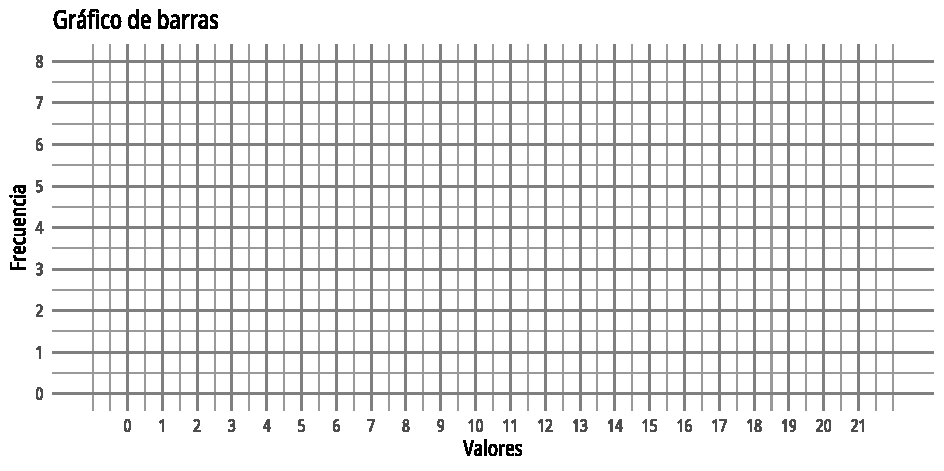
\includegraphics{grafico_vacio_1.pdf}\end{center}

\subsection{}
Usando los resultados anteriores, responda las siguientes preguntas
\begin{tasks}[label={\tcbox[colback=black!60, colframe=black!60, coltext=white, on line, boxsep=0pt, left=3pt, right=3pt, top=2pt, bottom=2pt]{\sffamily\bfseries\alph*}},
item-indent=1.2cm,column-sep=20pt,label-offset=0.3cm,label-width=15pt,after-item-skip=10pt]
    \task! ¿Cuánto vale la media (promedio) de los datos? ¿Qué significa que tenga este valor? \begin{lineas}[height=1.5cm]\end{lineas}
    \task! ¿Cuánto vale la mediana de los datos? ¿Qué significa que tenga este valor? \begin{lineas}[height=1.5cm]\end{lineas}
    \task! ¿Cuál es el rango de los datos? ¿Qué significa que tenga este valor? \begin{lineas}[height=1.5cm]\end{lineas}
    \task! ¿Cuánto vale el primer cuartil de los datos? ¿Qué significa que tenga este valor? \begin{lineas}[height=1.5cm]\end{lineas}
    \task! ¿Cuánto vale el tercer cuartil de los datos? ¿Qué significa que tenga este valor? \begin{lineas}[height=1.5cm]\end{lineas}
    \task! ¿A qué valor corresponde el percentil del 90\%? ¿Qué significa que tenga este valor? \begin{lineas}[height=1.5cm]\end{lineas}
\end{tasks}
\subsection{}

Haga un diagrama de caja usando los datos anteriores.
\begin{center}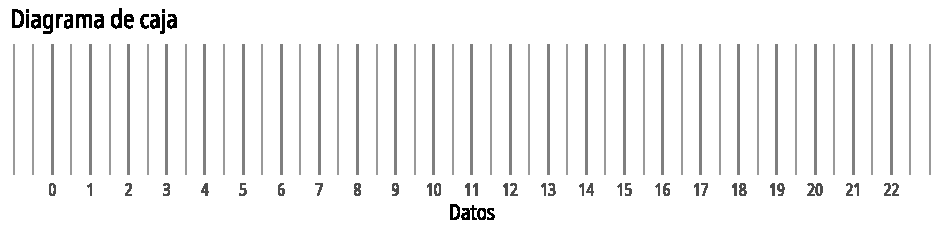
\includegraphics{diagrama_caja_vacio_1.pdf}\end{center}

\newpage\section*{Soluciones}
\setcounter{subsection}{0}
\subsection{}

\begin{center}\begin{tblr}{colspec={ccccc},hlines,vlines,hline{2,Z} = {1}{-}{},hline{2,Z} = {2}{-}{},row{even}={black!10}}
  .&Frecuencia&Probabilidad&Frecuencia Acumulada&Probabilidad Acumulada \\
 1&2&0.036&2&0.036 \\
 2&1&0.018&3&0.054 \\
 3&1&0.018&4&0.072 \\
 4&3&0.055&7&0.127 \\
 5&2&0.036&9&0.163 \\
 6&3&0.055&12&0.218 \\
 7&6&0.109&18&0.327 \\
 8&7&0.127&25&0.454 \\
 10&4&0.073&29&0.527 \\
 11&8&0.145&37&0.672 \\
 12&3&0.055&40&0.727 \\
 13&4&0.073&44&0.8 \\
 14&2&0.036&46&0.836 \\
 15&2&0.036&48&0.872 \\
 16&2&0.036&50&0.908 \\
 17&1&0.018&51&0.926 \\
 18&2&0.036&53&0.962 \\
 19&1&0.018&54&0.98 \\
 21&1&0.018&55&0.998 \\
 \end{tblr}\end{center}
\subsection{}
\begin{center}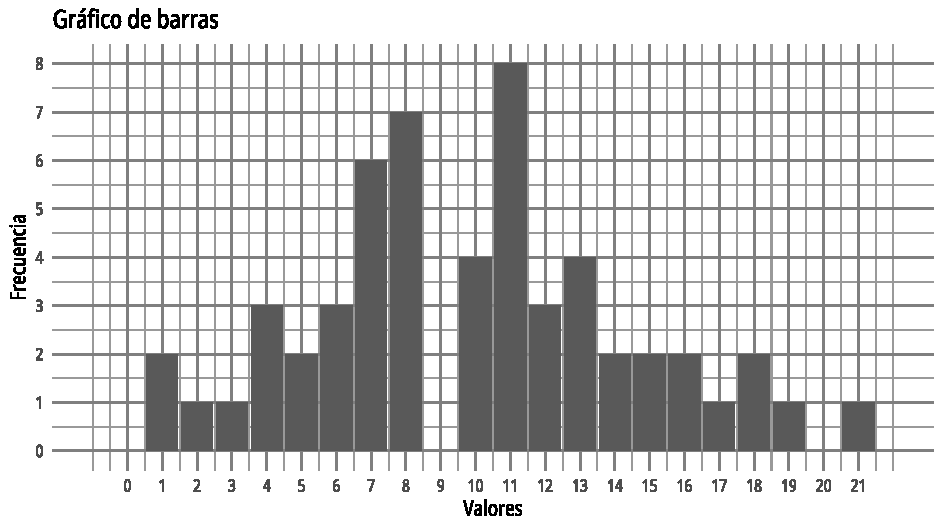
\includegraphics{grafico_barras_1.pdf}\end{center}
\subsection{}
\begin{tasks}[label={\tcbox[colback=black!60, colframe=black!60, coltext=white, on line, boxsep=0pt, left=3pt, right=3pt, top=2pt, bottom=2pt]{\sffamily\bfseries\alph*}},
item-indent=1.2cm,column-sep=20pt,label-offset=0.3cm,label-width=15pt,after-item-skip=10pt,item-format=\raggedright](2)\task La media es 9.891.
 Esto significa que los valores más frecuentes son los que están cercanos a 9.891, y es donde también se encuentran las barras más altas 
 en el gráfico de barras.\task La mediana es 10. 
 Esto significa que la mitad (50\%) de los datos tiene un valor menor 
 o igual a 10.\task El rango de los datos es 20. Esto 
 significa que la distancia entre el máximo (21) y el mínimo (1) de los datos es 20.\task El primer cuartil es 7. Esto significa que un cuarto de los datos (25\%) tiene un valor 
 menor o igual a 7.\task El tercer cuartil es 13. Esto significa que tres cuartos de los datos (75\%) tiene un valor menor
 o igual a 13.\task El percentil del 90\% es 16. Esto significa que el 90\% de los datos tiene un valor menor o igual a 16.\end{tasks}
\subsection{}
\begin{center}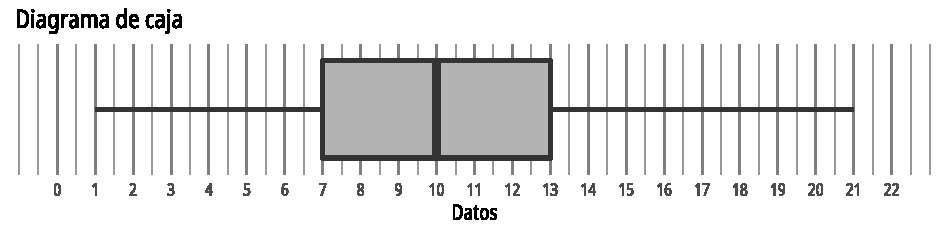
\includegraphics{diagrama_caja_1.pdf}\end{center}
\end{document}
